%energieEffizienz.tex
\section{Stand der globalen Energietransformation}
	\begin{frame}
	\frametitle{Stand: Net Zero Roadmap}
	\framesubtitle{\hspace*{\fill}iea (International Energy Agency)\cite{iea_net_zero2023}}
	
	\begin{itemize}
	 \item saubere Energietechnologien 
		  \begin{itemize}
			  \item verändern die Aussichten für Emissionen 
		    \item durch politische Maßnahmen, expandierende Märkte und sinkende Kosten
				\item selbst unter den derzeitigen politischen Rahmenbedingungen
		\end{itemize}
		\pause
		\item Verringerung der  Emissionen  voraussichtl. um \textbf{7,5 Gt } in 2030    
			 \begin{itemize}
		   	 \item bezogen auf das  Basisszenario vor Paris aus dem Jahr 2015
			   \item Szenario STEPS (Stated Policies Scenario)  
				 \item 5 Gt  Ausbau der Photovoltaik und der Windkraft und 
				 \item fast 1 Gt durch  Elektrofahrzeuge 
			 \end{itemize}
			\pause
			\item  die prognostizierte Erwärmung von 2,4 $^\circ$C im Jahr 2100 \textbf<2->{besorgniserregend} hoch 
			\begin{itemize}
				\item unter den derzeitigen politischen Rahmenbedingungen 
				\item \textbf<2->{aber} um 1 $^\circ$C niedriger liegt als vor dem Pariser Abkommen im Jahr 2015.
     \end{itemize}
	\end{itemize}
		
	\end{frame}	
		

\begin{frame}{Stand: Net Zero Roadmap}
	\framesubtitle{\hspace*{\fill}iea (International Energy Agency)\cite{iea_net_zero2023}}
	\begin{center}
			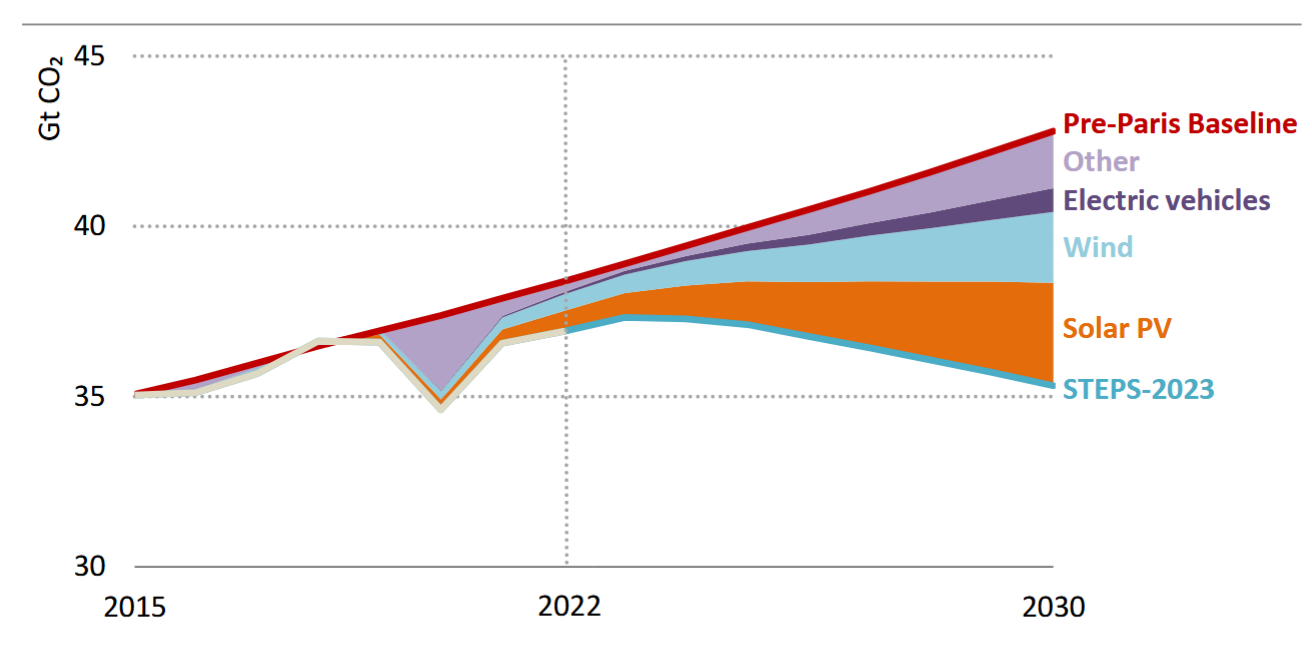
\includegraphics[width=.75\textwidth]{../Figures/global-energy-sector-co2-emissions-in-the-pre-paris-baseline-and-stated-policies-scenarios-2015-2030.png}
			
    \end{center}
	
\vfill

	\href{https://www.iea.org/reports/net-zero-roadmap-a-global-pathway-to-keep-the-15-0c-goal-in-reach/progress-in-the-clean-energy-transition}{\tiny https://www.iea.org/reports/net-zero-roadmap-a-global-pathway-to-keep-the-15-0c-goal-in-reach/progress-in-the-clean-energy-transition}
	\end{frame}	
		
\begin{frame}{AR6 Synthesis Report: Climate Change 2023}
\framesubtitle{\hspace*{\fill} \href{https://www.ipcc.ch/report/sixth-assessment-report-cycle/}{\tiny https://www.ipcc.ch/report/sixth-assessment-report-cycle/}}
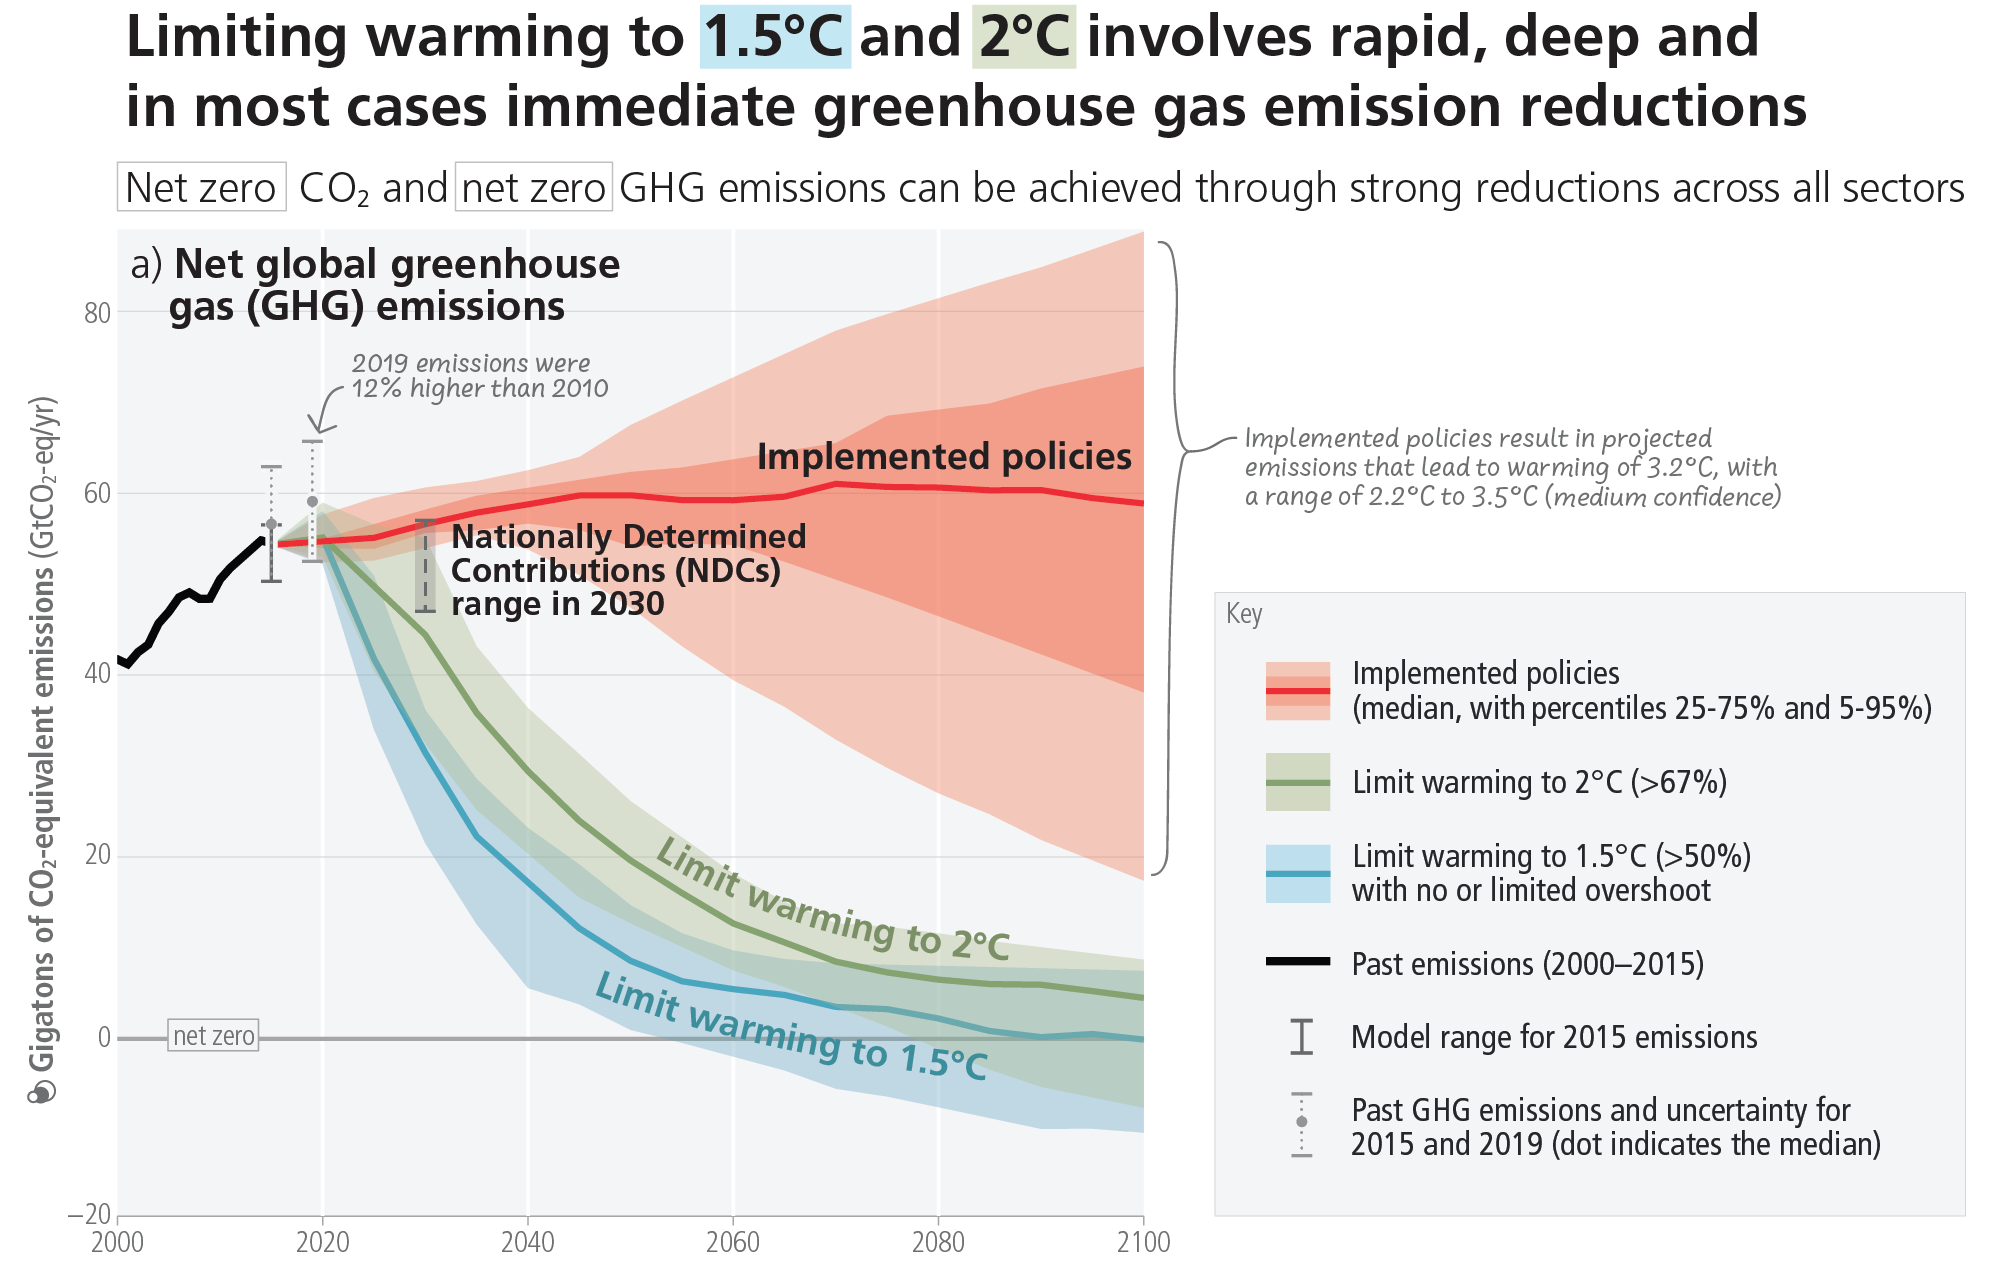
\includegraphics[width=1.00\textwidth]{../Figures/IPCC_AR6_SYR_SPM_Figure5.png}


\end{frame}


\section{\COz \ und  IT}

\begin{frame}{Auswirkungen digitaler Technologien}
%
\textbf{Digitale Technologien verursachen 2\% \hspace*{\fill}
                      der energiebezogenen Treibhausgasemissionen (THG)}
		\begin{itemize}
				\item direkte Auswirkungen auf Energieverbrauch und Emissionen
					\begin{itemize}
						\item rund 330 Mt \COze \ in 2020 
						\item durch Rechenzentren, Datenübertragungsnetze und vernetzten Geräte 
						\item 0,9\% der energiebezogenen THG-Emissionen  
				 \end{itemize}
			\pause
			\item geringe Steigerung der Emissionen seit 2010
				\begin{itemize}
					\item trotz der schnell wachsenden Nachfrage   
					\item Verbesserungen der Energieeffizienz, 
					\item Kauf von erneuerbaren Energien durch IKT-Unternehmen 
					\item umfassendere Dekarbonisierung der Stromnetze 
				\end{itemize}
				\pause 
			\item Aber \textbf<4->{Halbierung der Emissionen bis 2030}  für  Netto-Null-Emissionen bis 2050 (NZE) Szenario 
		\end{itemize}
		
\href{https://www.iea.org/energy-system/decarbonisation-enablers/digitalisation\#tracking}{\tiny https://www.iea.org/energy-system/decarbonisation-enablers/digitalisation\#tracking}

\end{frame}

\begin{frame}{Energieverbrauch IT in Deutschland  \cite{grunwald_energy_2022} S.2}
	\begin{center}
	     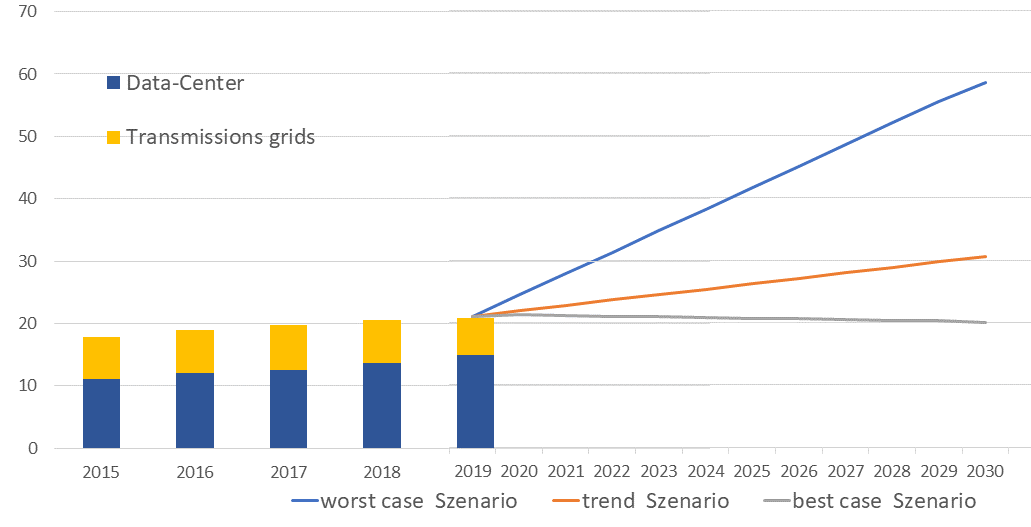
\includegraphics[width=.8\textwidth]{../Figures/fignachTAB22.png}
			
	\end{center}

\end{frame}

\section{Digitaler \COz-Fußabdruck im Alltag}

\begin{frame}{Wie sieht mein digitaler \COz-Fußabdruck aus?}
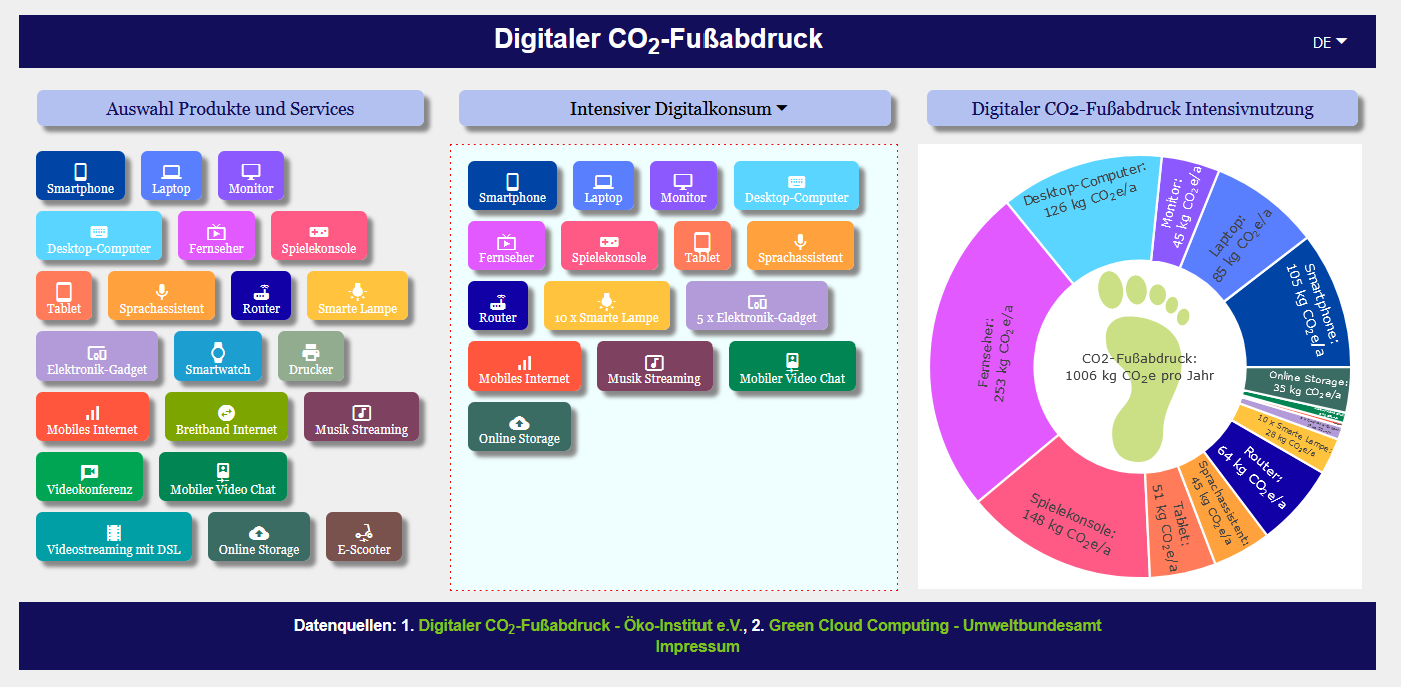
\includegraphics[width=1.00\textwidth]{../Figures/digit_CO2_FussAbruck.png}
Kann jeder für sich selbst unter \href{https://www.digitalcarbonfootprint.eu/}{https://www.digitalcarbonfootprint.eu/} bestimmen.

\end{frame}

\begin{frame}{Wie sieht mein digitaler Fußabdruck aus?}
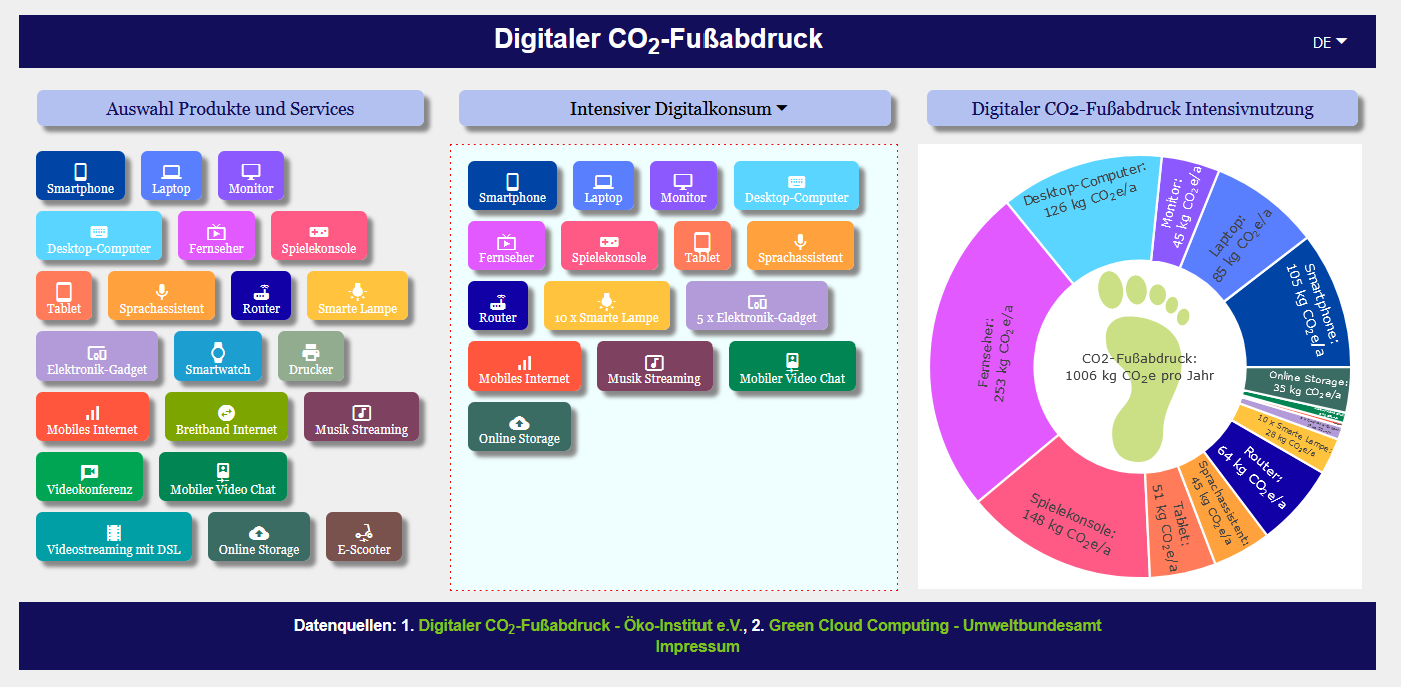
\includegraphics[width=1.00\textwidth]{../Figures/digit_CO2_FussAbruck.png}
Kann jeder für sich selbst unter \href{https://www.digitalcarbonfootprint.eu/}{https://www.digitalcarbonfootprint.eu/} bestimmen.

\end{frame}


\begin{frame}{Wie sieht mein digitaler Fußabdruck aus?}
		\begin{center}
			 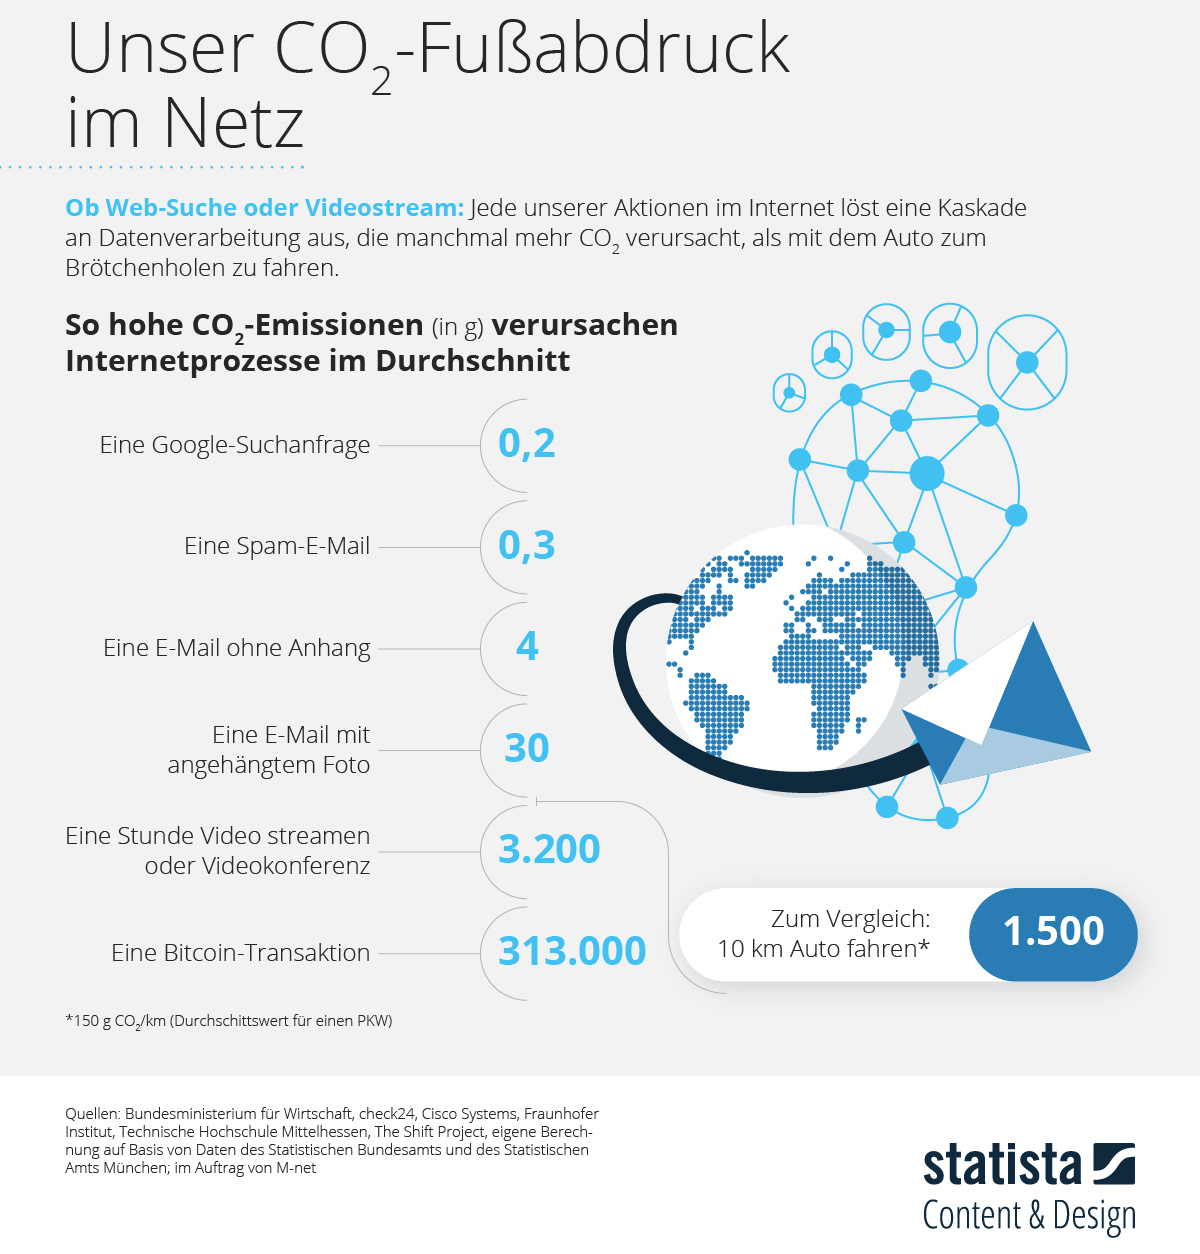
\includegraphics[width=.85\textwidth]{../Figures/grafik-co2-fussabdruck-internet.jpg}
			
		\end{center}
		
 \href{https://www.enviam-gruppe.de/energiezukunft-ostdeutschland/verbrauch-und-effizienz/stromverbrauch-internet}% 
{\tiny https://www.enviam-gruppe.de/energiezukunft-ostdeutschland/verbrauch-und-effizienz/stromverbrauch-internet}

\end{frame}		
\begin{frame}{Was kann ich tun?}
		\begin{center}
		   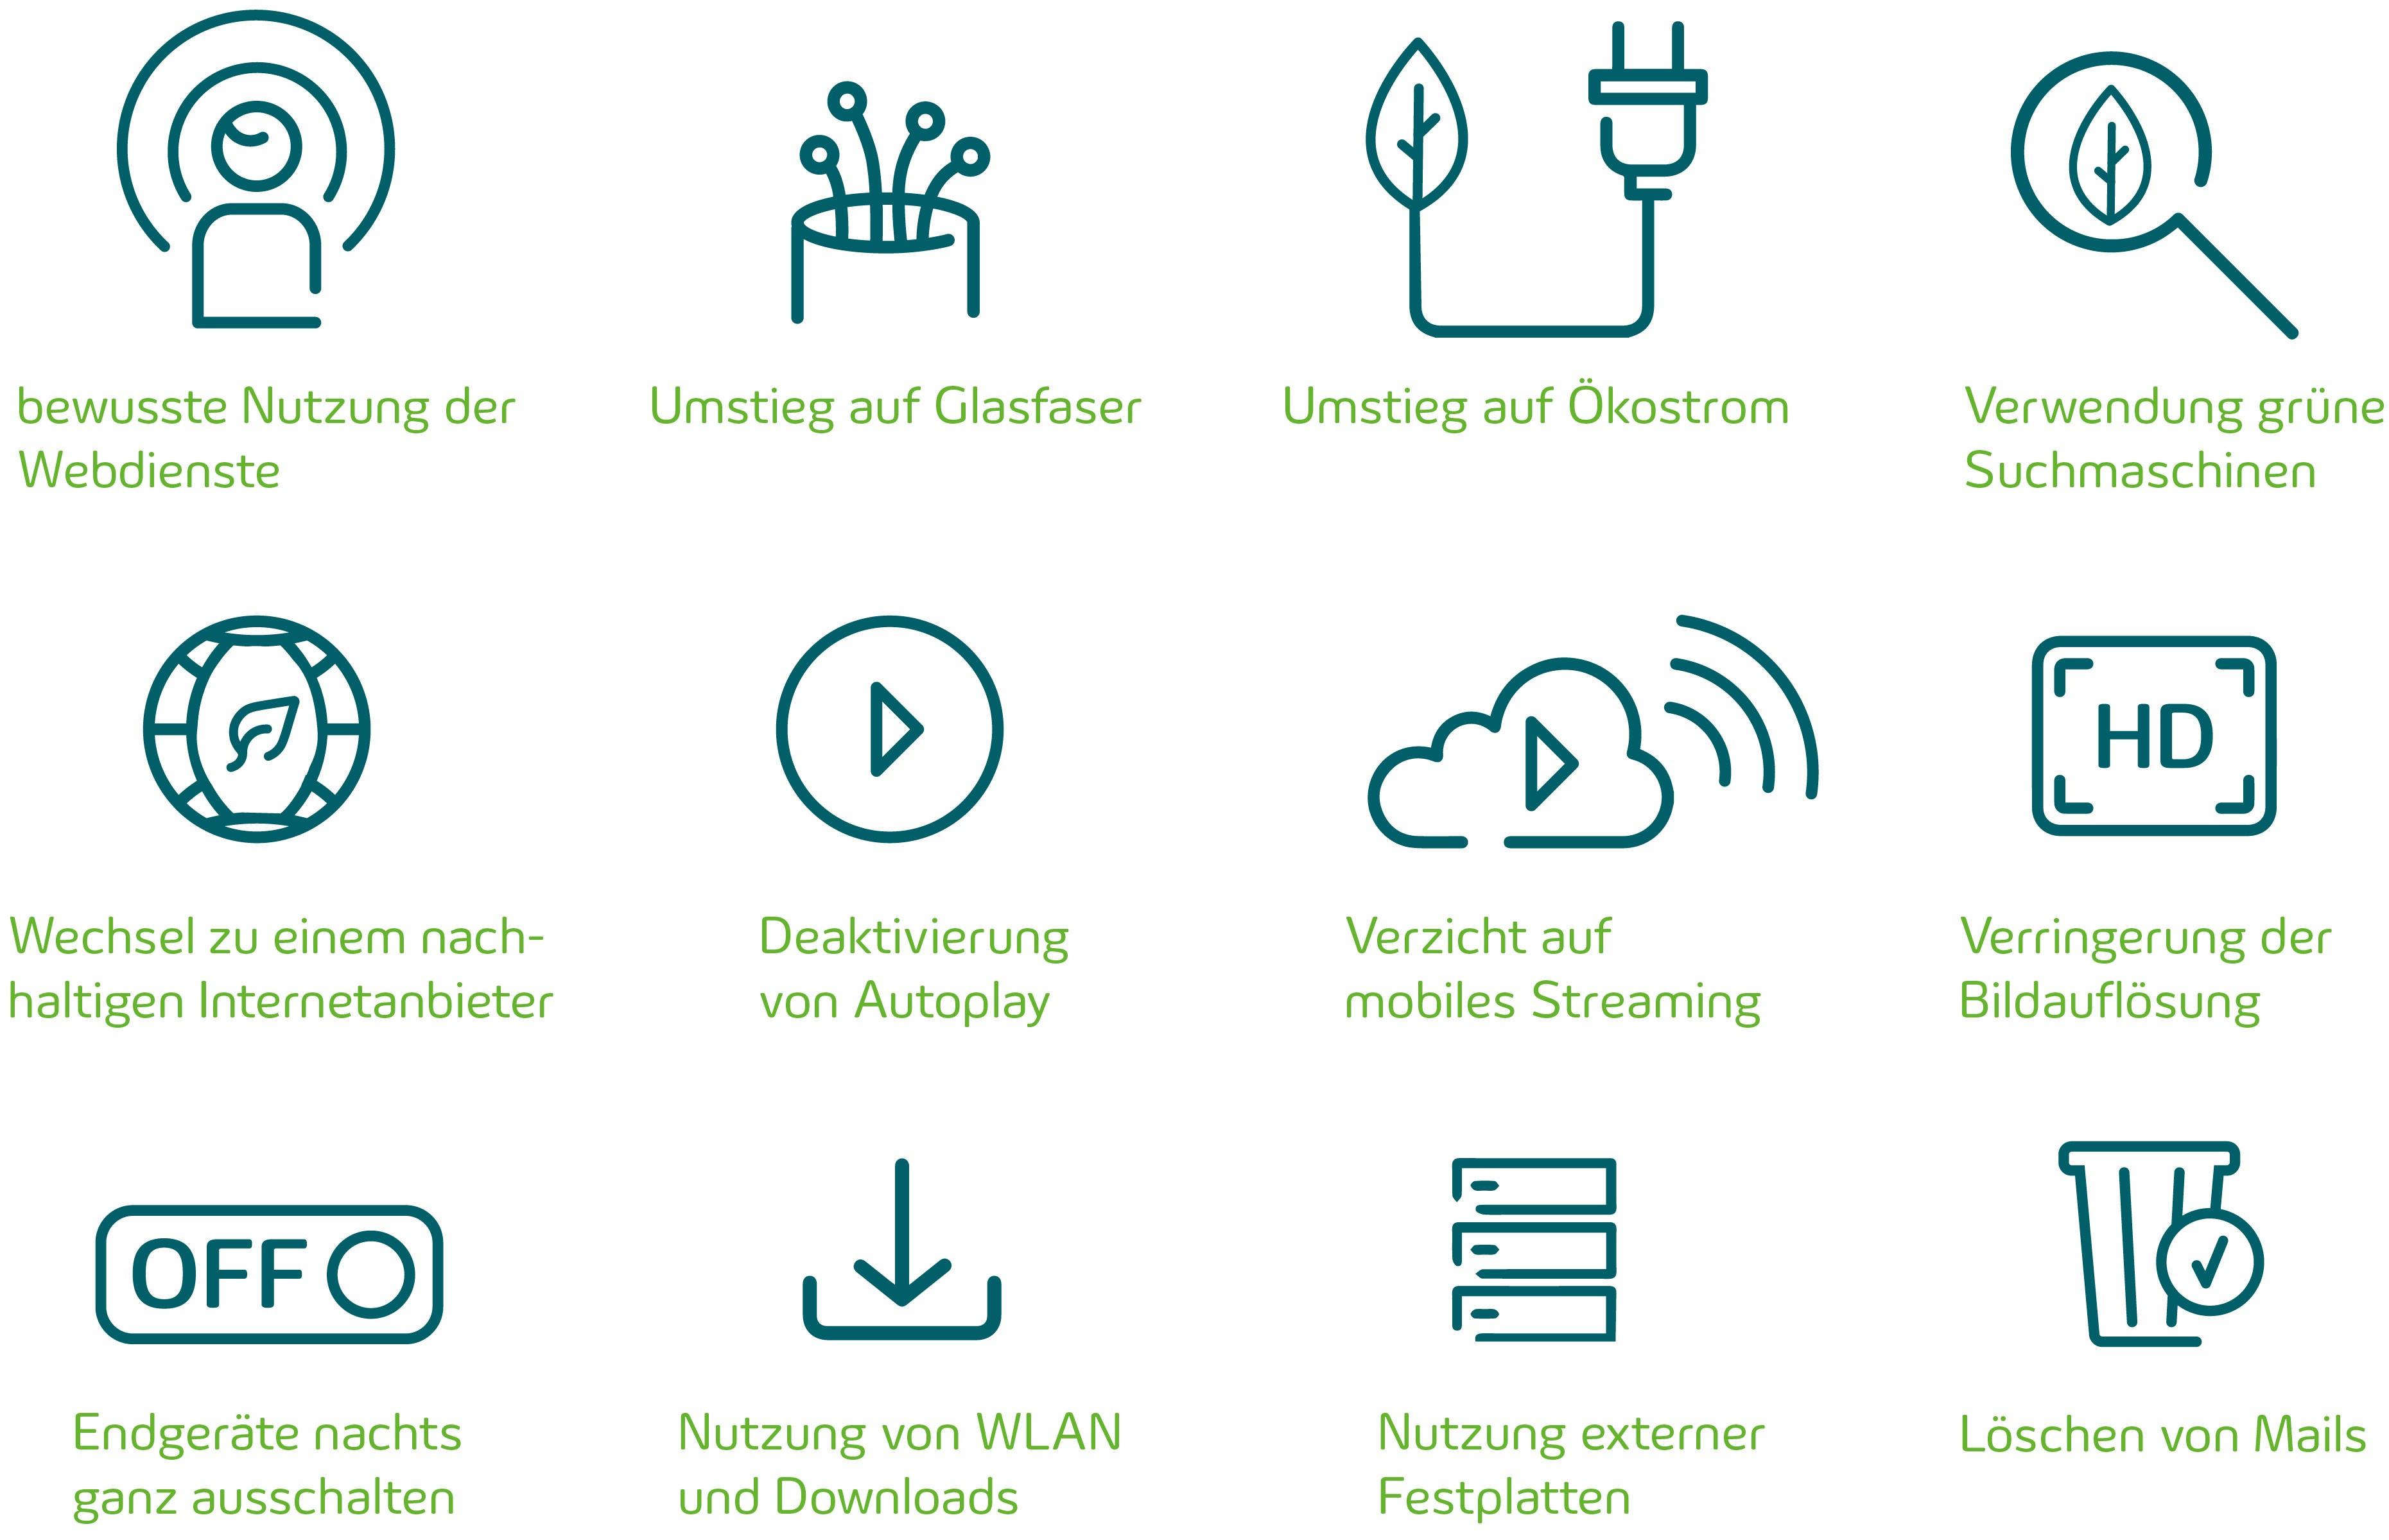
\includegraphics[width=.9\textwidth]{../Figures/grafik-nachhaltige-internetnutzung.jpg}
		\end{center}
		
 \href{https://www.enviam-gruppe.de/energiezukunft-ostdeutschland/verbrauch-und-effizienz/stromverbrauch-internet}% 
{\tiny https://www.enviam-gruppe.de/energiezukunft-ostdeutschland/verbrauch-und-effizienz/stromverbrauch-internet}

\end{frame}		

\section{(\COz-) effiziente Software}

\begin{frame}{Was ist kohlendioxid- (\COz-) effiziente Sofware}
	\framesubtitle{\hspace*{\fill}oder grüne, nachhaltige, ressourcen-effiziente....SW}
	\begin{block}{}
	Im Softwarebereich besteht unsere Rolle bei der Lösung des Klimaproblems \textbf<2->{wenigstens} 
	in der Entwicklung kohlendioxid-effizienter Anwendungen. 
	
	Kohlendioxid-Effizienz bedeutet, Anwendungen zu entwickeln,\textbf<2->{ die uns oder unseren  
	Nutzern den gleichen Mehrwert bieten}, aber weniger Kohlendioxid \COz \ ausstoßen.
	\end{block}\pause 
	~\\[-10mm]\hspace*{\fill}
	\href{https://www.freepngimg.com/png/77530-emoticon-thinking-thought-world-whatsapp-day-emoji}{%	
	
\includegraphics[width=3cm]{../Figures/emoji-thought.png}}
	%Lydia Simmons
	% Creative Commons (CC BY-NC 4.0) 
	%
\end{frame}

\begin{frame}{Digitale Suffizienz (\cite{santarius_digital_2023})} 
Grundlage dafür,  wie IKT zum  grundlegenden ökologischen Wandels beitragen kann 
\begin{itemize}
	\item Hardwaresuffizienz: \\
	   weniger Geräte produzieren \\
		ihr absoluter Energiebedarf so gering wie möglich
  \item  Softwaresuffizienz:\\
	   Datenverkehr und die Hardwareauslastung während der Anwendung so gering wie möglich
 \item Nutzersuffizienz:\\
      digitale Geräte sparsam einsetzen \\
			IKT in einem nachhaltigen Lebensstil nutzen
\item Ökonomische Suffizienz:\\
    Digitalisierung für  Übergang zu einer Wirtschaft mit
		Wirtschaftswachstum nicht mehr als primäres Ziel, \
		ausreichende Produktion und ausreichenden Verbrauch innerhalb der planetarischen Grenzen
\end{itemize}

\end{frame}

\begin{frame}{Kohlendioxid-effiziente Softwareentwicklung}

\begin{itemize}
	\item ressourcenschonende und 
	\item \emph{energie-effiziente Softwareprodukte}
	\item auf älterer Hardware laufend und 
	\item  auf älterer Hardware  zu aktualisieren
	\item mit einem hohen Maß an Transparenz und Autonomie
\end{itemize}

\end{frame}


\begin{frame}{\COz-effiziente Software}
\framesubtitle{\href{https://learn.greensoftware.foundation/measurement}{https://learn.greensoftware.foundation/measurement}}
		\begin{overprint}
			 \onslide<1>	  
				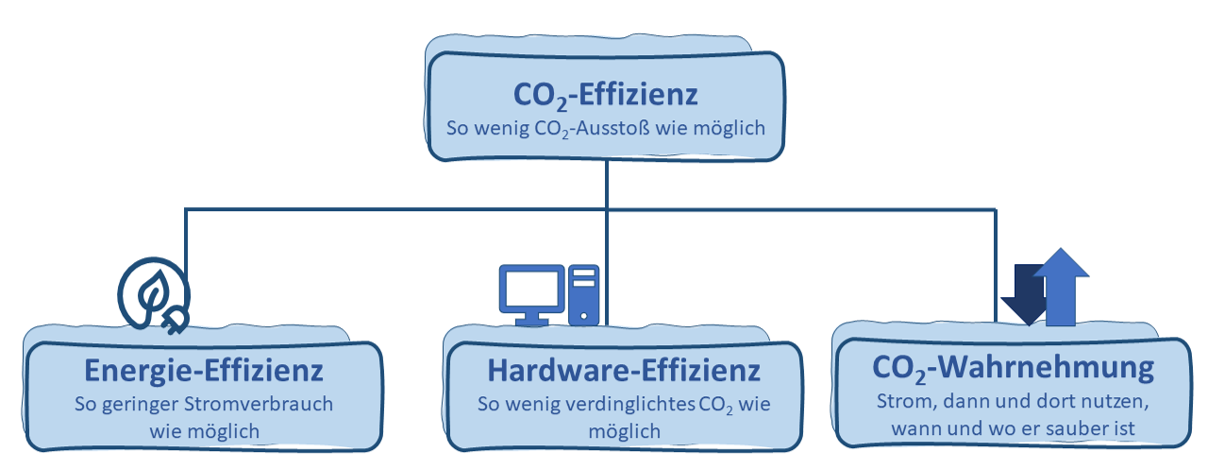
\includegraphics[width=1.00\textwidth]{../Figures/CO2awa_1.png}
			 \onslide<2>	  
				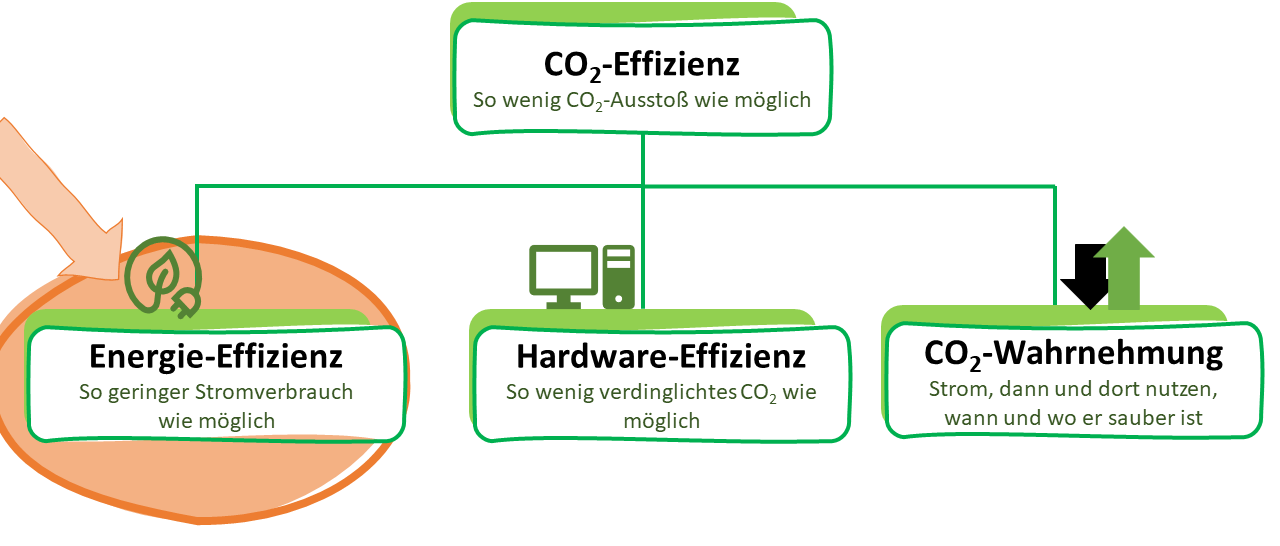
\includegraphics[width=1.00\textwidth]{../Figures/CO2awa_2.png}				
		\end{overprint}
\end{frame}


\begin{frame}
\frametitle{\COz-effiziente Software}
\framesubtitle{\href{https://learn.greensoftware.foundation//}{https://learn.greensoftware.foundation/}}
\begin{itemize}
     \item \COz-Effizienz: so wenig \COz~  wie möglich
		 \begin{itemize}
         \item \textbf<2->{Energieeffizienz: möglichst wenig Strom} 
         \item Hardware-Effizienz:  mit möglichst wenig (neuer) Hardware
         \item \COz-Wahrnehmung:  Strom mit der geringsten \COz-Emission
     \end{itemize}
		\pause
    \item Energieproportionalität: Maximierung  der  Energieeffizienz der Hardware
    \item Networking: Reduktion der Datenmenge und der Entfernung im  Netzwerk
    \item Demand Shaping:  \COz-bewusste Anwendungen bevorzugen
    \item \textbf<2->{Messungen: Was man nicht messen kann, kann man auch nicht verbessern.} 
		\item Verpflichtung zum Klimaschutz: Verstehen und umsetzen von Maßnahmen zur \COz-Reduktion
\end{itemize}
\end{frame}

\section{Experiment}

\begin{frame}
\frametitle{Messung}
\framesubtitle{\href{https://learn.greensoftware.foundation/measurement}{https://learn.greensoftware.foundation/measurement}}
\begin{block}{Idee}
What you can't measure, you can't improve.
\end{block}

\pause
\vfill 

Es gibt im groben drei Parameter, die -- unabhängig von der Infrastruktur -- die die \COz-Emissionen beeinflussen:

\begin{itemize}
	\item \textbf<3->{{Wieviel wird Energie verbraucht?}	   }   
				\begin{itemize}
					\item Messungen durch spezifische Werkzeuge, 
					\item wie JoularJX, Power Gadget etc
\end{itemize}
   \item Wie ist der  Energie-Mix (erneuerbar, fossil)
	\begin{itemize}
		\item der aktuelle oder auch der durchschnittliche
	\end{itemize}
    \item Wieviel Hardware wird benötigt?
\end{itemize}

\end{frame}


\begin{frame}{Laufzeit- und Energieeffizienz}

  Zusammenhang und Unterschiede
	    \begin{itemize}
		    \item Laufzeiteffizienz: Geschwindigkeit und Leistung von Computersystemen\\ Komplexität von Algorithmen\\Qualität der Implemetierung
        \item Energieeffizienz: Verbrauchte Energie eines Systems \cite{brown_toward_2010}
        \item \textbf<2->{Keine direkte Proportionalität?? }\\
		           Verbesserte Laufzeiteffizienz bedeutet nicht unbedingt verbesserte Energieeffizienz und umgekehrt?
							
							\begin{itemize}
								\item[Ja]  Direkter Zusammenhang zwischen Energieeffizienz und Performance 
								           \cite{pereira_energy_2017,cascaval_folklore_2014,pinto_energy_2017}\\
													  dann reicht vermutlich die Laufzeitmessung
													
								\item[Nein] Kein direkzer Zusammenhang zwischen Energieeffizienz und Performance 
								      \cite{trefethen_energy-aware_2013,lima_haskell_2016} \\
											dann sind neuartige Messungen nötig
							\end{itemize}
		\end{itemize}
							
\end{frame}


\begin{frame}{Energiemessung von Software}
\framesubtitle{Mikromodul Energiemessung von und durch Software}

Wieso  Software-Tools und nicht mit Hardware-Tools :
\begin{itemize}
    \item die Kosten 
    \item der Aufwand
    \item und nicht jedes System kann einfach an der Steckdose gemessen werden\\
		          wie zum Beispiel bei batteriebetriebenen Geräten 
\end{itemize}
\end{frame}

\begin{frame}{JoularJX}
\framesubtitle{Mikromodul Energiemessung von und durch Software}
~\\\hspace*{\fill}

\includegraphics[width=0.40\textwidth]{../Figures/joular.png}

\begin{itemize}
	\item JoularJX ist ein Software-Energieüberwachungstool
  \item Hilfe für  Softwareentwickler, um den Stromverbrauch 
ihrer Programme zu verstehen und zu analysieren

\end{itemize}
\end{frame}

\begin{frame}{PowerJoular}
\framesubtitle{Mikromodul Energiemessung von und durch Software}

\includegraphics[width=0.90\textwidth]{../Figures/powerjoular.png}

\begin{itemize}
	\item Überwachung des Stromverbrauchs des Computers mithilfe RAPL-Schnittstelle.
	\item fürLinux (x86 und Raspberry Pis)
	\item Hardwareunterstützung zur Erfassung des Stromverbrauch 
\end{itemize}
in GitHub: \href{https://github.com/joular/powerjoular}{https://github.com/joular/powerjoular}\\
Mehr Infos : \href{https://joular.github.io/powerjoular/}{https://joular.github.io/powerjoular/}

\hspace*{\fill} \cite{noureddine-ie-2022}
\end{frame}

\begin{frame}{Softwarefootprint.py}
\framesubtitle{Mikromodul Energiemessung von und durch Software}
Skript, dass
\begin{itemize}
	\item   die Prozessstatistiken nach dem Vorkommen  bestimmten Befehle durchsucht,
	\item  deren CPU-Laufzeiten addiert,
	\item  und daraus Energieverbrauch und Treibhausgasemissionen der Software berechnet
	\item für den lokalen Computer.
\end{itemize}

in GitHub \href{https://github.com/oekoj/softwarefootprint}{https://github.com/oekoj/softwarefootprint}
\end{frame}


\begin{frame}{Intel Power Gadget}\begin{columns}
\framesubtitle{Mikromodul Energiemessung von und durch Software}
\column{8cm}


\begin{itemize}
  \item  Schätzung der Leistung auf Softwareebene\\
	       ohne H/W-Instrumentierung 
	\item zusätzliche Funktionen wie die Schätzung \\
	         des Stromverbrauchs bei Systemen mit mehreren Sockeln 
	\item extern aufrufbare APIs zur Extraktion von \\
	           Stromverbrauchsinformationen in Codeabschnitten
	\item  Tool  integrierbar in Codeabschnitte 
\end{itemize}
\column{4cm}
~\\[-32mm]\hspace*{\fill}
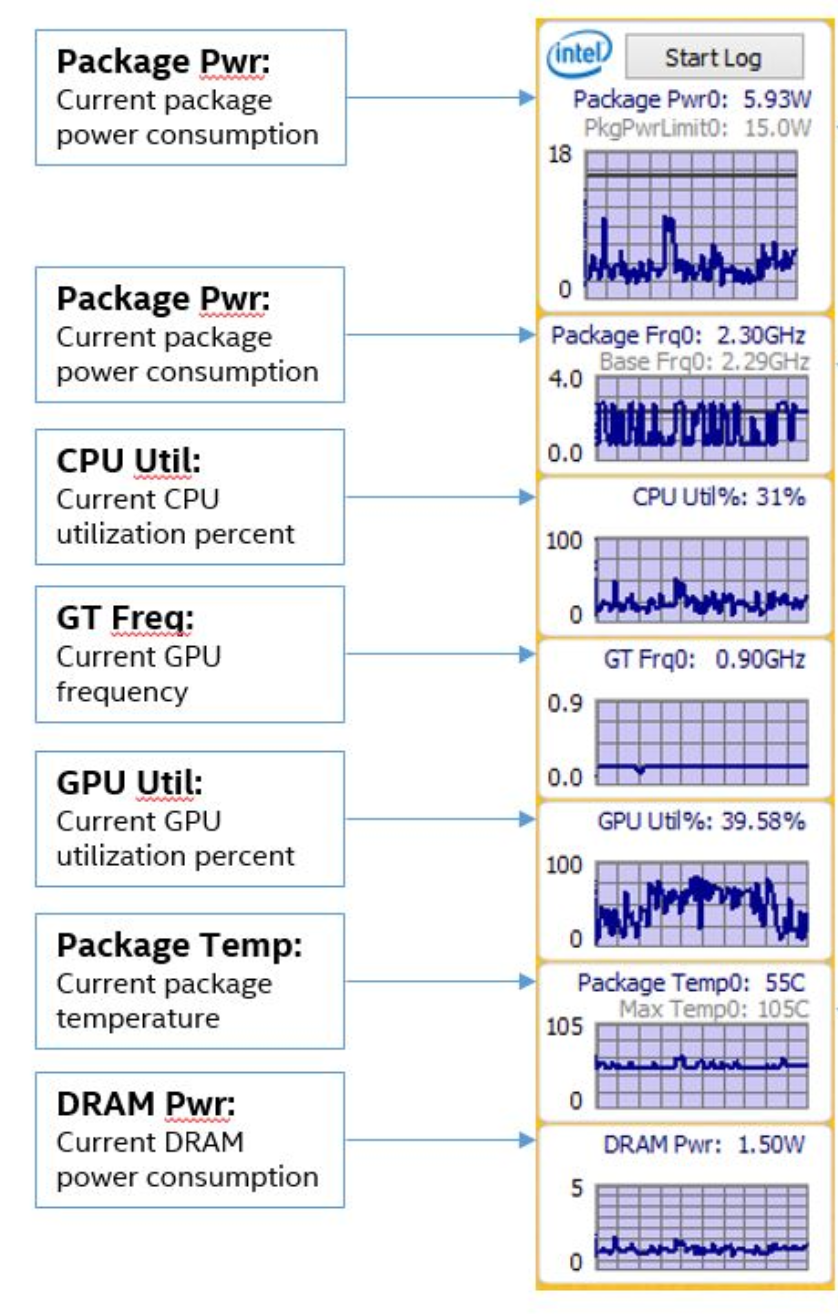
\includegraphics[width=4cm]{../Figures/PowerGadget.png}


\end{columns}
\end{frame}

\begin{frame}{Hardware-Monitore}
\framesubtitle{Mikromodul Energiemessung von und durch Software}
\begin{itemize}
	\item HWMonitor  \href{https://www.cpuid.com/softwares/hwmonitor.html}%
	                      {\tiny https://www.cpuid.com/softwares/hwmonitor.html}
		
		\begin{itemize}
			\item  für Windows auf x86
			\item ermöglicht die Messung des Gesamtstromverbrauchs eines Computers
			\item  ein Hardware-Überwachungsprogramm, für\\
			   Spannungen, Temperaturen, Leistungen, Ströme, Lüftergeschwindigkeiten, Auslastungen, Taktfrequenzen
			\item keine spezifischen Funktionen zur Überwachung einzelner Prozesse oder Programme.
		\end{itemize}
												

\item Open Hardware Monitor  \href{https://openhardwaremonitor.org/}{\tiny https://openhardwaremonitor.org/}
\begin{itemize}
	\item funktioniert auf Windows und auf Linux mit Einschränkungen\\ \hspace*{\fill}
	        da es dort teilweise weniger Sensorinformationen bereitstellt
					
   \item  ähnlich dem HWMonitor
	\item  ermöglicht primär die Messung des Gesamtstromverbrauchs eines Computers
			\item keine spezifischen Funktionen zur Überwachung einzelner Prozesse oder Programme
\end{itemize}
\end{itemize}
\end{frame}


\begin{frame}{Experiment: Energieeffizienz}
\begin{itemize}
	\item Mögliche Aufgaben\\
	      Feststellung der Energieeffizienz\\
				Vergleich Laufzeit vs. Energieeffizienz
\begin{itemize}
	\item z.B. TSP mit Minimaler-Spannbaum-Heuristik
	\item z.B. \textbf<2->{Eulerkreise}
\end{itemize}
	\item erster Schritt zur ressourceneffizienten Softwareentwicklung 
	\item JUNIT-Tests für die Messung 
	\begin{itemize}
		\item  des Energieverbrauchs
		\item  der Laufzeit
\end{itemize}
	\item Erstellung einer Tabelle  (csv-Datei)  mit
	\begin{itemize}
		\item Spalten unterschiedlich grossen Datensätzen
		\item Hardware
		\item IDE
		\item Java-Version
			
\end{itemize}
\end{itemize} 
\end{frame}

\section{Ausblick}
\begin{frame}{Ausblick: Energieproportionalität \cite{wong_retrospective_2015}}
		%\begin{columns}
		%\column{8cm}
				\begin{itemize}
					\item Verhältnis von Leistungsverbrauch zur nützlichen Arbeit
					\item  Energieproportionalität als Brücke zwischen Zeit- und Energieeffizienz
				\item Einsatz Energieproportionalität
				 \begin{itemize}
					 \item Verbesserte Energieeffizienz 
					 \item Reduzierte Kosten 
					 \item \textbf<2->{nicht für als Maßeinheit für Implementierungen }\\sondern nur für gesamte Systeme sinnvoll
					\end{itemize}
			\end{itemize}
		%	
		%\column{5cm}
		\hspace*{2cm}
		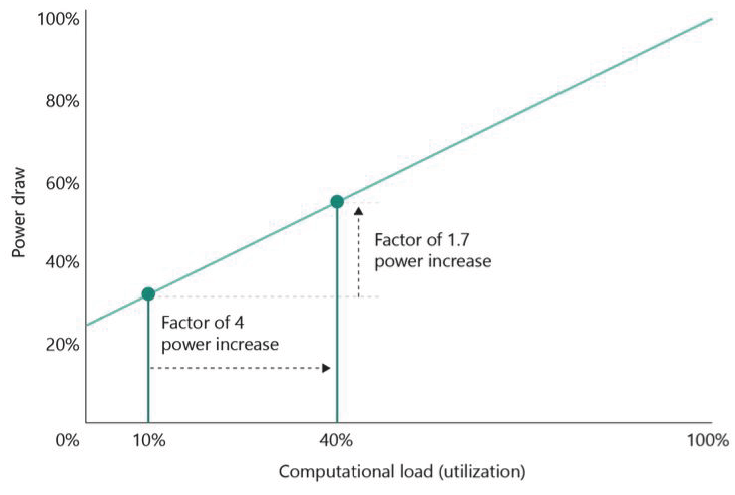
\includegraphics[width=.65\linewidth]{../Figures/energiePropor.png}
		\hspace*{\fill}\\
		\hspace*{\fill} \href{https://learn.microsoft.com/en-us/training/modules/sustainable-software-engineering-overview/}%
		               {\tiny https://learn.microsoft.com/en-us/training/modules/sustainable-software-engineering-overview/}
		%\end{columns}
\end{frame}
